\chapter{\textbf{Literature review}}  \label{chapter:lit}

According to Chowdhury, (2003) “Natural Language Processing (NLP) is an area of research and application that explores how computers can be used to understand and manipulate natural language text or speech to do useful things. NLP researchers aim to gather knowledge on how human beings understand and use language so that appropriate tools and techniques can be developed to make computer systems understand and manipulate natural languages to perform desired tasks” (Chowdhury, 2003, p.1).\\

One of the advantages of utilising documents, texts, and minutes, is the possibility of working with quantitative and qualitative data at same time (Bholat et al., 2015, p.1). Working with both types of data it is possible to carry out studies and statistical inferences that would not be possible with just structured data – even though the applicability of these type of study is vast, it has only been used in economics for a short time.\\

Recently, Shapiro, Sudhof \& Wilson (2020) reported that an economic index, created by the authors, based on sentiment analysis from economic papers was related with macroeconomic variables. For this paper the authors consider real variables as real interest rate, inflation, domestic consumption, and real growth domestic product for the American economy. They evaluated whether the index score would be related to the behaviour of these variables.

\begin{figure}[!h]
    \centering
    \caption{Impulse response of a positive news sentiment shock on economic activity}
    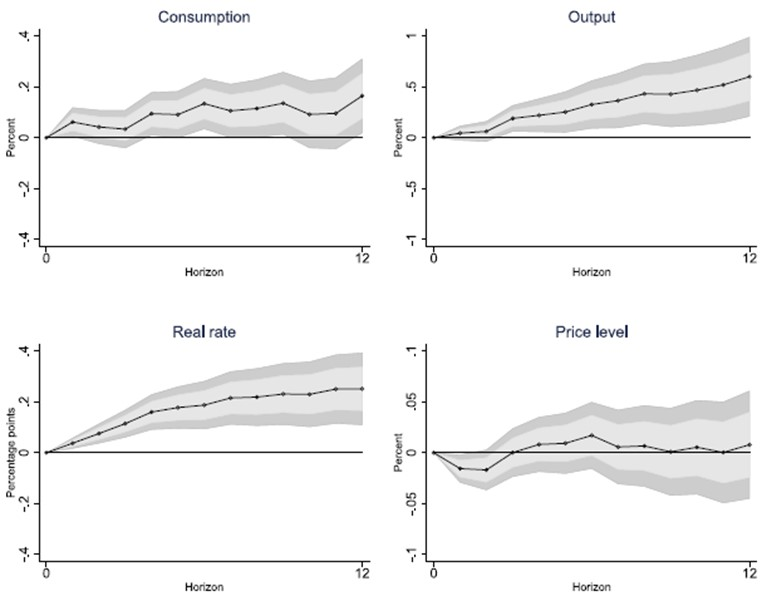
\includegraphics[width=.8\textwidth]{images/image1.jpg}
    \caption*{Source: \cite[p.16]{shapiro2020measuring}}
    \label{fig:my_label}
\end{figure}

Utilising statistical and econometrics technics, specifically the Vector Autoregressive (Sims, 1980), the authors showed by the impulse response function that it is possible to understand what happens to the economy when considering the score of the index: given a positive shock at the index sentiment score, it affects positively the consumption, the interest rate, and the output. The effect at the price level, however, is transitory while the persistence of the shock at the other variables gradually gets higher: “Extending the horizon out further […] indicates that the responses of consumption, output, and the real rate peak between 12 and 18 months after the shock before gradually waning” \citet[p.16]{shapiro2020measuring}.\\
\cite
Another study tried to estimate the central bank objectives using text analysis \cite{shapiro2021taking}. This time the authors sought to understand the main objective of a central bank (Federal Reserve Board) utilising its internal discussions (U.S. Federal Open Market Committee’s - FOMC). They implemented a model with the aim of incorporating text analysis in structural estimations in order to take into account the “weights” of the central banker’s preferences. An index of negativity was created based on a dictionary \cite{loughran2011liability} of economic terms in order to implement a new approach to estimate the parameters of a central bank objective function: for each hearing of the FOMC was created a score based in the frequency of positive and negative word of the hearing. The result presented by the authors is that usually the models do not consider those preferences, thus the incorporation of such technics would significantly improve the models and its interpretations, helping to explain what is, in fact, the objective function of a central bank.\\

In order to complement the literature of sentiment analysis in economics, \cite{ostapenko2020macroeconomic} contributed analysing “how the change of tone or topic in newspaper affects the macroeconomy”. The author transformed articles from newspaper (employing a topic model and vector representation of documents with clustering) into time series and based on this time series, evaluated the sentiment of each article. On occasion, the article demonstrated that given a new shock in the sentiment of the articles, it could mean an increase over the long run, in output and consumption – it also affects the inflation and interest rate, however transiently.\\

Progressively, text mining, sentiment analysis and other techniques end up helping the field of economics to understand better what is happening and what is the relation of the conjunctural or structural scenarios with social expressions. Sentiment analysis helps to understand the consumption behaviour, or even how the media can influence or even chance an economic scenario. Text mining allows to extract qualitative and quantitative information from a text or a corpus. Sooner or later NLP will be increasingly used for a better understanding of the world or the field of economic science.\\

Overall, the approach of researchers and contributors in this area is particularly similar. In terms of estimations, there is a consensus on the importance of treating endogeneity related to macroeconomic relations: when a model is estimated, the use of an autoregressive vector is generally chosen, even if based on an unorthodox approach in the statistical field, considering from methods of Bayesian estimations to autoregressive vector with signal constraints \citet{santos2020indice}.\\

In terms of descriptive analysis, or in terms of classifiers, the approach varies according to the chosen methodology, generally with greater emphasis on classification techniques such as support vector machine, k-means neighbours, or k-nearest neighbour (KNN) \citet{ostapenko2020macroeconomic}. Still, it is worth noting that approaches that assume NLP techniques such as tokenization (see section 3) are still little used, especially with regard to estimations: it is important to emphasize that not using techniques such as tokenization in estimations can create a lack of results in terms of contribution to economic science, given the fact that a better understanding of what happens in the economic scenario is possible and plausible based on a better understanding of how terms and expressions are related to economic cycles.\\



